\chapter{Actividades}
\section{Introduccion}
\begin{flushleft}
	El diagrama de actividades un diagrama UML de comportamiento que muestra el flujo de control o el flujo de objetos, con especial énfasis en la secuencia y las condiciones de este flujo.
		\\
	Estos diagramas son utilizados para describir cualquier tipo de procesos, es especialmente común para modelar de forma gráfica los diferentes casos de uso, transacciones o procedimientos que haya en un sistema de información. En resumen, son utilizados para representar la forma en la que un sistema hace una implementación.
		\\
	Los diagramas de actividades muestran una secuencia de acciones, un flujo de trabajo que va desde un punto inicial hasta un punto final.
	\\
	
	
	
	
\end{flushleft}
	


\newpage
\begin{flushleft}
Por este motivo, en un diagrama de actividades aparecerán acciones y actividades correspondientes a distintas clases. Colaborando todas ellas para conseguir un mismo fin. A continuación, se muestra un diagrama de actividades de ejemplo para entender la notacion de dicho diagrama:
\begin{center}
	{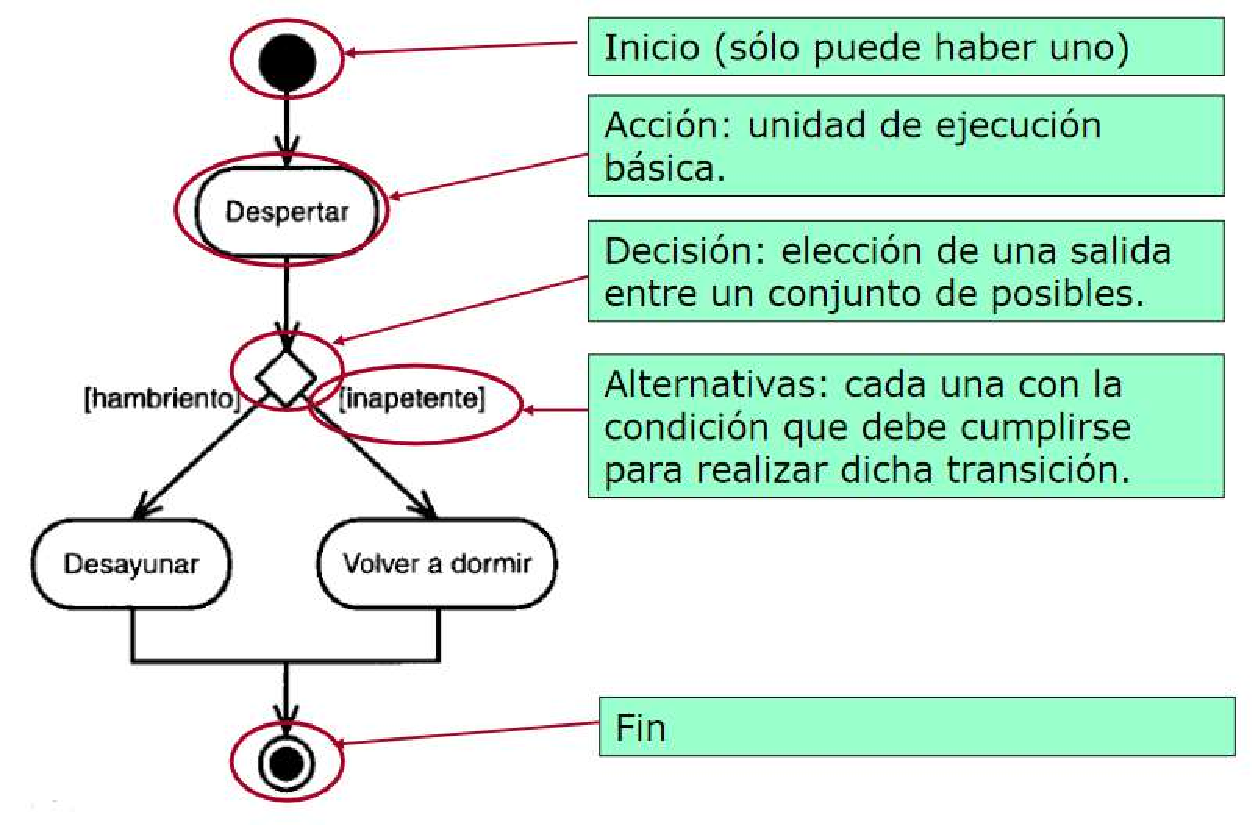
\includegraphics[width=1\linewidth]{imgs/DiagramaActividades-Algoritmo/EjemploDiagramaActividades}}
\end{center}
\end{flushleft}
\newpage
\section{Diagrama de Actividades - Algoritmo Tarifa}
\begin{flushleft}
	Para nuestro proyecto hemos diseñado un diagrama de Actividades en la herramienta Coloso, donde especificamos el flujo de actividades del algoritmo que se encarga de calcular la tarifa de alquiler de un espacio de parqueo dependiendo del tiempo que se vaya a ocupar.
	\\

	\begin{center}
		{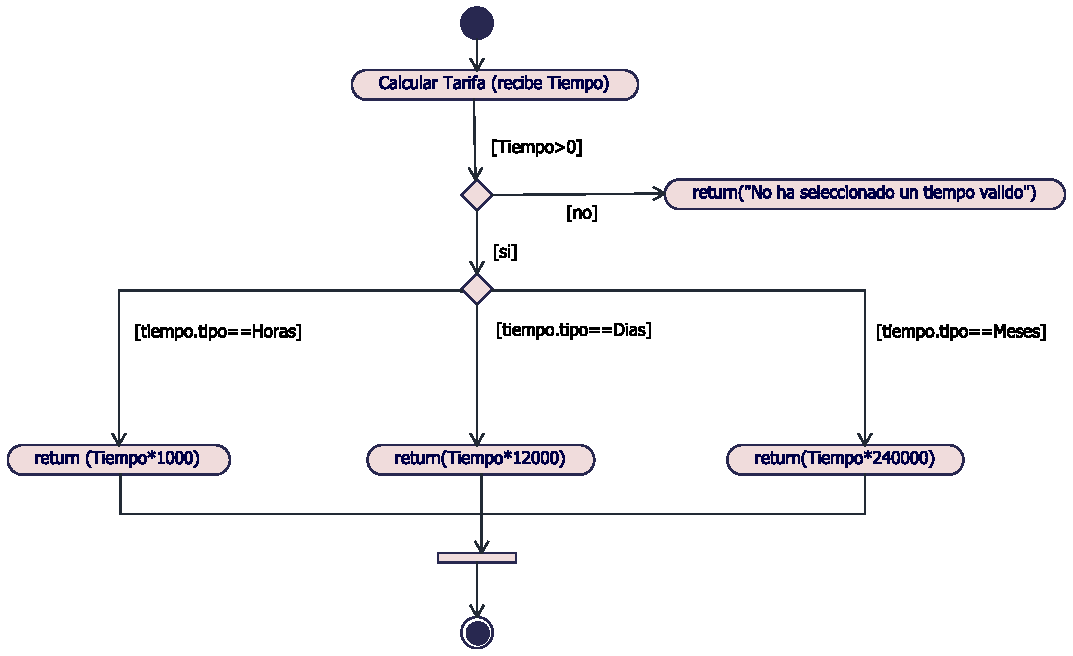
\includegraphics[width=1.18\linewidth]{imgs/DiagramaActividades-Algoritmo/DiagramaActividades-AlgoritmoTarifa}}
	\end{center}
	El diagrama muestra cómo se calcula la tarifa del parqueadero, inicia preguntándose si el tiempo es mayor que 1 en dado caso que no lo sea le retornara un mensaje diciendo que el tiempo no es válido, en caso de que el tiempo si sea mayor que 1, se elegirá en que periodo se va a operar el tiempo de parqueo, los cuales son horas, días o meses y con respecto a este periodo se le asigna un valor que al multiplicarlo con el tiempo termine dando la tarifa del parqueo (siendo, entre mayor periodo de uso de parqueo, mas economica sera la tarifa).
\end{flushleft}

\newpage
\section{WorkFlow}
\subsection{Diagrama de Actividades - WorkFlow}
\begin{flushleft}
	Un diagrama de Work Flow, o flujo de trabajo, es la representacion del proyecto utlizando la notacion del diagrama de actividades, con la diferencia que se definen particiones que van a actuar como Entidades, entidades que van a interactuar entre si con los distintos componentes de un diagrama de actividades convencional.
	\\
	A continuacion, la representacion en WorkFlow de nuestro proyecto:
	
	\begin{center}
		{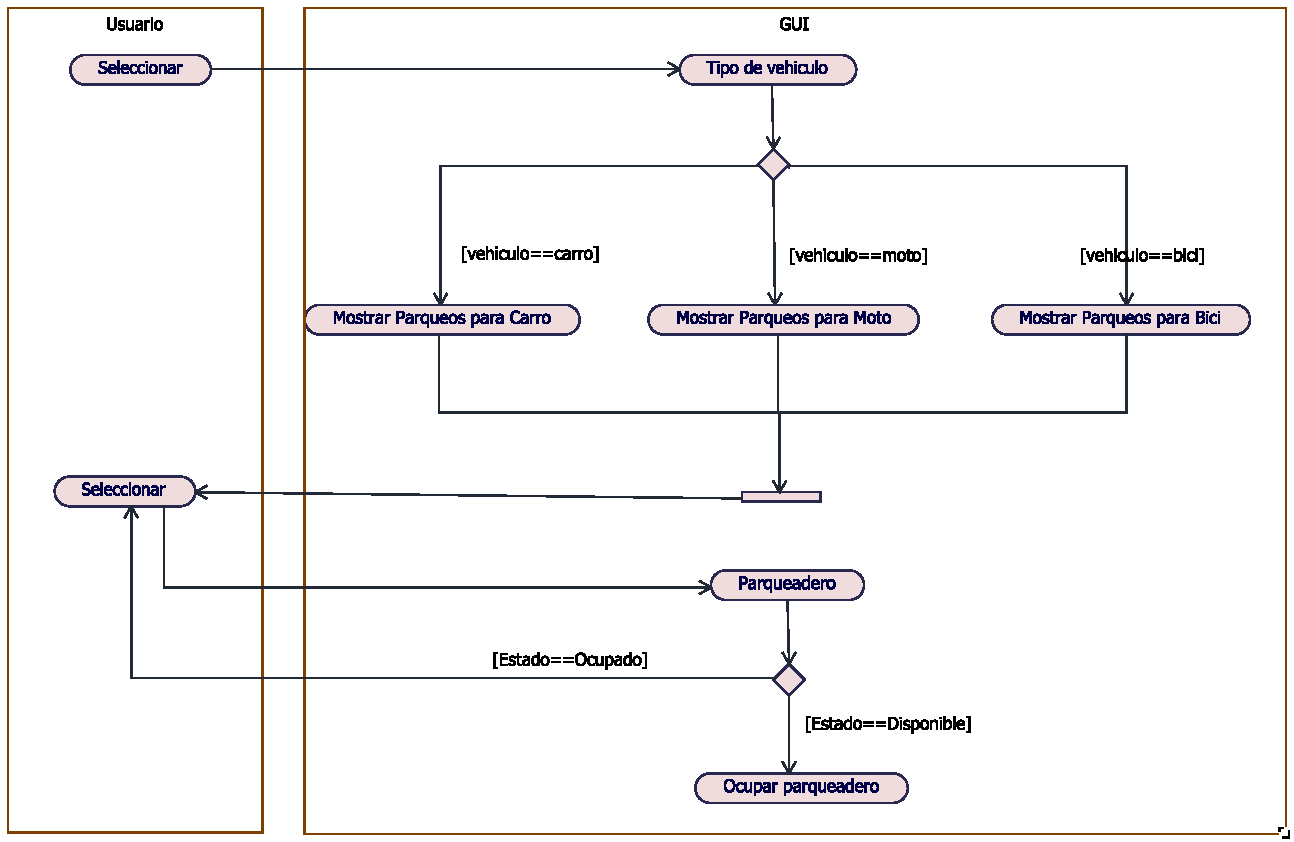
\includegraphics[width=1.20\linewidth]{imgs/DiagramaWorkFlow-Proyecto/WorkFlow-Proyecto}}
	\end{center}

	Como se puede apreciar en el diagrama este está dividido en dos particiones las cuales representan el usuario y la GUI del programa. Todo inicia cuando el usuario debe seleccionar el tipo de parqueaderos que necesita de acuerdo a su vehículo, esto lo hace por medio de la GUI la cual obtiene el tipo seleccionado y toma la decisión de mostrar de acuerdo al tipo de vehículo seleccionado los parqueaderos en el mapa, una vez este dato es sincronizado el usuario tendra la opcion de elegir un parqueadero en el mapa entre los obtenidos anteriormente a través del mapa. Ya habiendo seleccionado el parqueadero se verificará el estado tomando este como condición para saber qué decisión tomar siendo que si está disponible le permite parquear y actualizar el estado a ocupado, en caso contrario el usuario tendrá que volver a realizar el proceso de seleccionar un parqueadero.
\end{flushleft}